\documentclass[a4paper,11pt]{article}
\pdfoutput=1 % if your are submitting a pdflatex (i.e. if you have
             % images in pdf, png or jpg format)

\usepackage{jheppub} % for details on the use of the package, please
                     % see the JHEP-author-manual


\usepackage{hyperref}

\usepackage{amssymb,amsmath,amsfonts}
\usepackage{epsfig}
\usepackage{array}
%\usepackage{verbatim}

\usepackage{tikz}

\usetikzlibrary{calc,through,backgrounds,patterns,decorations.pathmorphing,decorations.markings,%
		trees,positioning,arrows,chains,shapes.geometric,%
    decorations.pathreplacing,shapes}

\usepackage{pgfplots}
%\usepgfplotslibrary{patchplots,fillbetween}

\usepgfplotslibrary{fillbetween}    
\pgfplotsset{compat=1.10}
%\usepackage[dvipsnames]{xcolor}


\usepackage{amsmath}
\usepackage{multirow}
\usepackage{array}
\usepackage{bm}

\newcommand{\vect}[1]{\boldsymbol{\mathbf{#1}}}

\newcommand{\CA}{\mathcal{A}}
\newcommand{\CB}{\mathcal{B}}
\newcommand{\CC}{\mathcal{C}}
\newcommand{\CD}{\mathcal{D}}
%\newcommand{\CE}{\mathcal{E}}
\newcommand{\CF}{\mathcal{F}}
\def\CJ{\mathcal{J}}
\newcommand{\CG}{\mathcal{G}}
\newcommand{\CL}{\mathcal{L}}
\newcommand{\CO}{\mathcal{O}}
\newcommand{\CN}{\mathcal{N}}
\newcommand{\CI}{\mathcal{I}}
\newcommand{\CT}{\mathcal{T}}
\newcommand{\CS}{\mathcal{S}}
\newcommand{\CM}{\mathcal{M}}
\newcommand{\CQ}{\mathcal{Q}}
\newcommand{\CE}{\mathcal{E}}
\newcommand{\CZ}{\mathcal{Z}}

\newcommand{\Z}{\mathbb{Z}}
\newcommand{\C}{\mathbb{C}}
\newcommand{\R}{\mathbb{R}}

\newcommand{\gym}{g_{\rm YM}}

\newcommand{\eps}{\epsilon}
\newcommand{\grad}{\vec{\nabla}}
\newcommand{\el}{\kappa}

\newcommand{\ads}{\mbox{AdS}}

\newcommand{\nn}{\nonumber}
\newcommand{\lspa}{\ \ ,\ \ \ \ }
\newcommand{\spa}{\ , \ \ }

\newcommand{\ds}{\displaystyle}

\newcommand{\tr}{\mathop{{\rm Tr}}}
\DeclareMathOperator{\sgn}{sgn} \DeclareMathOperator{\diag}{diag}

\newcommand{\vecto}[2]{\left( \begin{array}{c} #1 \\ #2 \end{array}
\right) }
\newcommand{\matrto}[4]{\left( \begin{array}{cc} #1 & #2 \\
#3 & #4 \end{array} \right) }
\newcommand{\vectre}[3]{\left( \begin{array}{c} #1 \\ #2\\ #3 \end{array}
\right) }
\newcommand{\matrtre}[9]{\left( \begin{array}{ccc} #1 & #2 & #3 \\ #4 & #5 & #6 \\ #7 & #8 & #9 \end{array} \right) }


\newcommand{\hB}{{}^* \! B}
\newcommand{\hC}{{}^* \! C}
\newcommand{\hF}{{}^* \! F}
\newcommand{\hJ}{{}^* \! J}

\newtheorem{definition}{Definition}[section]
\newtheorem{proposition}[definition]{Proposition}
\newtheorem{theorem}[definition]{Theorem}
\newtheorem{lemma}[definition]{Lemma}
\newtheorem{corollary}[definition]{Corollary}
\newtheorem{comment}[definition]{Comment}
\newtheorem{example}[definition]{Example}
\newtheorem{conjecture}[definition]{Conjecture}

\newcommand{\proof}{\noindent {\bf Proof:}\ }
\newcommand{\squ}{\noindent $\square$}

\newcommand{\bin}[2]{\Big( \begin{array}{c} #1 \\[-1mm] #2 \end{array}
\Big) }

\def\Tr{\mathrm{Tr}}

%---------------------------------------------------------
\numberwithin{equation}{section}
%---------------------------------------------------

\begin{document} 
?
\section{intro}
\subsection{some formula}
\begin{figure}[h!]
\centerline{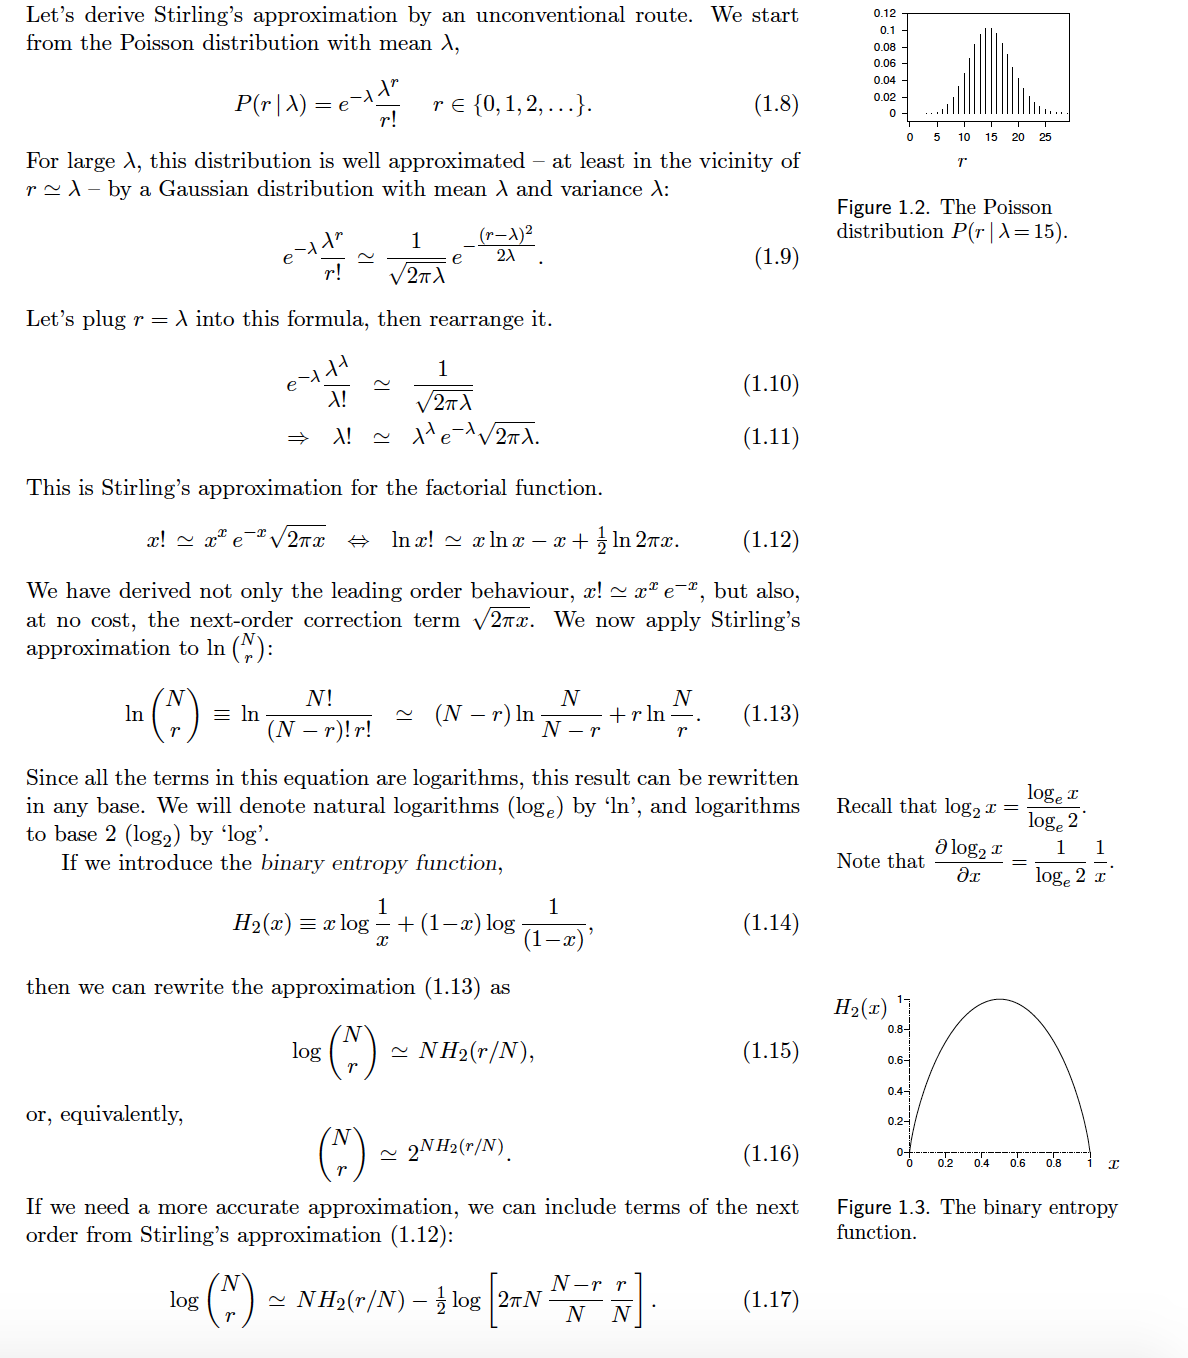
\includegraphics[scale=0.6]{probability_formulae.png}}
\caption{Some formula}
\end{figure}

\subsection{assumptions in inference}

First, once assumptions are made, the inferences are objective and unique,
reproducible with complete agreement by anyone who has the same information
and makes the same assumptions. For example, given the assumptions
listed above, $\mathcal{H}$, and the data D, everyone will agree about the posterior probability
of the decay length
$$
P(\lambda | D, \mathcal{H})= {P(D|\lambda , \mathcal{H})P(\lambda |  \mathcal{H}) \over P(D|\mathcal{H})}
$$

Second, when the assumptions are explicit, they are easier to criticize, and
easier to modify { indeed, we can quantify the sensitivity of our inferences to
the details of the assumptions.



Third, when we are not sure which of various alternative assumptions is
the most appropriate for a problem, we can treat this question as another
inference task. Thus, given data D, we can compare alternative assumptions
$\mathcal{H}$ using Bayes' theorem

$$
P( \mathcal{H}|D,I)= {P(D| \mathcal{H},I)P(\mathcal{H}|I) \over P(D|I)},
$$
where I denotes the highest assumptions, which we are not questioning.

Fourth, we can take into account our uncertainty regarding such assumptions
when we make subsequent predictions. Rather than choosing one particular
assumption $\mathcal{H}^*$, and working out our predictions about some quantity $t$,
$P(t |D, \mathcal{H},I)$, we obtain predictions that take into account our uncertainty 
about H by using the sum rule
$$
P({\textbf t} | D, I)= \Sigma_{\mathcal{H}} P({\textbf t}|D, \mathcal{H},I)P( \mathcal{H}|D,I) 
$$

This is another contrast with orthodox statistics, in which it is conventional
to `test' a default model, and then, if the test `accepts the model' at some
`significance level', to use exclusively that model to make predictions.
{\it probability theory reaches parts that ad hoc methods cannot reach.}



Model comparison as inference. Assume we have two hypotheses. In order to perform model comparison, We wish to
know how probable $P(\mathcal{H}_1)$ is given the data. By Bayes' theorem,

$$
P( \mathcal{H}_1|{\textbf s},F)= {P(s|F, \mathcal{H}_1)P(\mathcal{H}_1) \over P({\textbf s}|F)},
$$
and 
$$ 
P( \mathcal{H}_0|{\textbf s},F)= {P({\textbf s}|F, \mathcal{H}_0)P(\mathcal{H}_0) \over P({\textbf s}|F)}
$$

The normalizing constant in both cases is the total probability of geting the observed data. and 
$$
P(s|F)=P({\textbf s}|F, \mathcal{H}_1)P(\mathcal{H}_1) +P({\textbf s}|F, \mathcal{H}_0)P(\mathcal{H}_0)
$$

To evaluate the posterior probabilities of the hypotheses we need to assign
values to the prior probabilities $P(\mathcal{H}_1)$ and $P(\mathcal{H}_0)$; in this case, we might
set these to 1/2 each. And we need to evaluate the data-dependent terms
$P(s|F, \mathcal{H}_1)$ and $P(s|F,\mathcal{H}_0)$. We can give names to these quantities. The
quantity $P(s|F, \mathcal{H}_1)$  is a measure of how much the data favour $ \mathcal{H}_1)$, and we
call it the evidence for model $ \mathcal{H}_1)$. {\it How model comparison works : The evidence for a model is usually the normalizing constant of an earlier Bayesian inference.}

\section{Clustering}
\subsection{Motivation of clustering}
First, a good clustering has
predictive power. Second, clusters can be a useful aid to communication because they allow
lossy compression. A third reason for making a cluster model is that failures of the cluster
model may highlight interesting objects that deserve special attention. A fourth reason for liking clustering algorithms is that they may serve
as models of learning processes in neural systems.

\subsection{K-means}
The K-means algorithm is an algorithm for putting N data points in an M-dimensional space into K clusters. Each cluster is parameterized by a vector
${\textbf m}^{(k)}$ called its mean. 

First of all, set K means {${\textbf m}^{(k)}$} to random values. In the assignment step, each data point n is
assigned to the nearest mean. 
$$
\hat k^{(n)} = argmin_k d({\textbf m}^{(k)}, {\textbf x}^{(n)})
$$
An alternative, equivalent representation of this assignment of
points to clusters is given by `responsibilities', which are indicator
variables $r^{(n)}_k$. In the assignment step, we set $r^{(n)}_k$ to one if mean k is the closest mean to datapoint $ {\textbf x}^{(n)}$; otherwise, $r^{(n)}_k$ is zero.
$$
r^{(n)}_k = \{
\begin{array}{cc}
1 ~~~~~~if ~\hat k^{(n)}=k\\
0 ~~~~~~if ~\hat k^{(n)}\ne k\\
\end{array}
$$
In the update step, the means are adjusted to
match the sample means of the data points that they are responsible for. The update step is very similar to how to find the center of the mass in physics. 
$$
{\textbf m}^{(k)}= {\Sigma_n ~ r^{(n)}_k {\textbf x}^{(n)} \over R^{(k)}}
$$
where $R^{(k)}$ is the total responsibility of mean $k$
$$
R^{(k)}=\Sigma_n~r^{(n)}_k
$$









\subsection{Exercise 22.5}
$$
P(k_n = 1|x_n, \vect{\theta})= {P(x_n|k_n=1,\vect{\theta})P(k_n=1,\vect{\theta}) \over P(x_n,\vect{\theta})}
$$
$$
= {P(x_n|k_n=1,\vect{\theta})P(k_n=1,\vect{\theta}) \over \Sigma_{k_n}  P(x_n|k_n=1,\vect{\theta})P(k_n=1,\vect{\theta}) +P(x_n|k_n=2,\vect{\theta})P(k_n=2,\vect{\theta}) }
$$
where $\vect{\theta}=\mu_k, ~\sigma_k$. 
$$
P(k_n=1,\vect{\theta}) \equiv p_1,~~P(k_n=2,\vect{\theta}) \equiv p_2
$$

Then, 
$$
P(k_n=1|x_n,\vect{\theta})= {p_1 \over p_1+p_2 \exp[-(w_1x_n+w0)]}
$$
$$
P(k_n=2|x_n,\vect{\theta})= {p_2 \over p_2+p_1 \exp[-(w_1x_n+w0)]}
$$
where $w_1=2(\mu_1-\mu_2)$, $w_0=-(\mu_1-\mu_2)(\mu_1+\mu_2)$

$$
P(k_n=k|x_n,\vect{\theta}) \equiv p_{k|n}
$$


By assumption, the prior probability $p_1=p_2=1/2$ then, (22.17) of the book is satisfied. 
$$
L\equiv \log \Pi_n P(x_n|\{\mu_k\},~\sigma)
$$
$$
{\partial \over \partial{\mu_k}}L = \Sigma_n  {p_{k|n} (x_n-\mu_k)\over \sigma^2}
$$
\section{Monte Carlo }



\end{document}








